
\documentclass[a4paper,12pt]{article}
\usepackage{graphicx}
\newenvironment{codeblock}{\fontfamily{ccr}\selectfont}{\par}

\title{
	\normalfont \normalsize 
	\textsc{Pimpri Chinchwad College of Engineering \\ 
		Computer Laboratory - III} \\
	[10pt] 
	\rule{\linewidth}{0.5pt} \\[6pt] 
	\huge Assignment No - 1\\
	\rule{\linewidth}{2pt}  \\[10pt]
}
\author{}
\date{\normalsize}


\begin{document}
\maketitle

%%%%%%%%%%%%%%%%%%%%%%%
% FOR A NUMBERED LIST
% \begin{enumerate}
% \item Your_Item
% \end{enumerate}
%%%%%%%%%%%%%%%%%%%%%%%
% FOR A BULLETED LIST
% \begin{itemize}
% \item Your_Item
% \end{itemize}
%%%%%%%%%%%%%%%%%%%%%%%
% TO IMPORT AN IMAGE
% \includegraphics[width=\textwidth]{name_of_file}
% \textwidth makes the picture the width of the paragraphs
%%%%%%%%%%%%%%%%%%%%%%%%%%%%%%
% TO CREATE A FIGURE WITH A NUMBER AND CAPTION
% \begin{figure}
% \includegraphics[width=\textwidth]{image}
% \caption{Your Caption Goes Here}
% \label{your_label}
% \end{figure}
% REFER TO YOUR FIGURE LATER WITH
% \ref{your_label}
% LABELS NEED TO BE ONE WORD
%%%%%%%%%%%%%%%%%%%%%%%%%%%%%
% TO ADD CODE
% \begin{codeblock}
% Some code in "courier" font
%\end{codeblock}
%%%%%%%%%%%%%%%%%%%%%%%%%%%%%
\section{Aim}
	\paragraph{}Write a program in python/ Java/ Scala/ C++/ HTML5 to implement password data encryption. Use encryption method overloading.
	
\section{Objective}
	\begin{itemize}
		\item To encrypt data using password for preventing unauthorized access.
	\end{itemize}
	
\section{Software Requirements}
	\begin{itemize}
		\item   Operating System:Windows 10, Ubuntu.
		\item	Java
	\end{itemize}
	
\section{Mathematical Model}
	\paragraph{} 
		S 	= {s, e, x, y, Fme, DD, NDD}  											\\\\
	S   =   Initial State  										\\
	E 	=   End State  																\\
	X	= Input Value\\
	    X=\{x1,x2\} \\
	  where,  x1=UserName\\
	    x2=Password\\
	Y	=Output\\
	Y=\{y1\}\\
	y1=\{"Successfully added into Database\}\\
	 Fme 	= 	Main function \\
	 Fme=\{f1\}\\f1="MD5 Algorithm to calulate Hash of the Password".\\
	 H=MD5(x2)\\
	 where, H=Hash of the Password.\\
	DD 	= 	Deterministic data \{username,password\}\\
	NDD	= 	Non Deterministic Data \{ Hash\}															\\
  
	
\section{Theory}
	
	\subsection{MD5}
	\begin{itemize}
	    \item 
MD5 algorithm can be used as a digital
signature mechanism.The MD5 message-digest algorithm is a widely used cryptographic hash function producing a 128-bit (16-byte) hash value, mostly expressed in text format as a 32-digit hexadecimal number. MD5 has been utilized in a variety of cryptographic applications and is also commonly used to verify data integrity.
	\end{itemize}

\subsection{Password Encryption}
Encryption is the most effective way to achieve data security. To read an encrypted file, you must have access to a secret key or password that enables you to decrypt it. Unencrypted data is called plain text ; encrypted data is referred to as cipher text.	\\

\subsection{Method Overloading}
Method Overloading is a feature that allows a class to have two or more methods having same name, if their argument lists are different.
\newline
\newline
\newline
\begin{verbatim}
 class CalHash{  
    
      String hash(String pass)
      {
      String hashcode=getHash(pass);
      return hashcode;
      }  
      
      String hash(String pass,StringSalt)
      {
      String hashcode = getHash(pass+salt);
      return hashcode;
      }  
      
      public static void main(String args[]){  
      CalHash obj=new CalHash();
      
      if(pass.length()<8)
        obj.hash(pass,salt); 
      else
        obj.hash(pass);  
      
      }  
    }  

\end{verbatim}
    

\subsection{Java Swing}
Swing API is set of extensible GUI Components to ease developer's life to create JAVA based Front End/ GUI Applications. It is build upon top of AWT API and acts as replacement of AWT API as it has almost every control corresponding to AWT controls. Swing component follows a Model-View-Controller architecture to fulfill the following criteria.
\begin{itemize}
  \item  A single API is to be sufficient to support multiple look and feel.

   \item API is to model driven so that highest level API is not required to have the data.

   \item API is to use the Java Bean model so that Builder Tools and IDE can provide better services to the developers to use it.
\end{itemize}

\textbf{CODE:}
\begin{verbatim}
 
package com.pratiksha.cl3.assignment1;

import javax.swing.*;

import java.awt.*;

import java.awt.event.*;

import java.sql.*;

public class Login extends JFrame implements ActionListener

{

	JLabel l1, l2, l3;

	JTextField tf1;

	JButton btn1;

	JPasswordField p1;
	JCheckBox checkbox;

	Login()

	{

		setTitle("Login Form in Windows Form");

		setVisible(true);

		setSize(800, 800);

		setLayout(null);

		setDefaultCloseOperation(JFrame.EXIT_ON_CLOSE);

		l1 = new JLabel("Login Form in Windows Form:");

		l1.setForeground(Color.blue);

		l1.setFont(new Font("Serif", Font.BOLD, 20));

		l2 = new JLabel("Enter Email:");

		l3 = new JLabel("Enter Password:");

		tf1 = new JTextField();

		p1 = new JPasswordField();

		checkbox = new JCheckBox("Security");

		btn1 = new JButton("Submit");

		l1.setBounds(100, 30, 400, 30);

		l2.setBounds(80, 70, 200, 30);

		l3.setBounds(80, 110, 200, 30);

		tf1.setBounds(300, 70, 200, 30);

		p1.setBounds(300, 110, 200, 30);
		
		checkbox.setBounds(300, 160, 100, 100);

		btn1.setBounds(150, 160, 100, 30);

		add(l1);

		add(l2);

		add(tf1);

		add(l3);

		add(p1);

		add(checkbox);

		add(btn1);

		btn1.addActionListener(this);

	}

	public void actionPerformed(ActionEvent e)

	{

		showData();

	}

	public void showData()

	{

		JFrame f1 = new JFrame();

		JLabel l, l0;

		String str1 = tf1.getText();

		char[] p = p1.getPassword();

		String str2 = new String(p);

		try

		{

			// set state
			checkbox.setSelected(true);

			// check state

			Class.forName("com.mysql.jdbc.Driver");
			Connection con = DriverManager.getConnection("jdbc:mysql://localhost:3306/test", "root", "root");
			PreparedStatement ps;
			if (checkbox.isSelected()) {
				ps = con.prepareStatement("select name from regform where user=? and passO=?");
				ps.setString(1, str1);
				String password = MD5Calculation.encrypt(str2, "MD5", str1);
				ps.setString(2, password);
			} else {

				ps = con.prepareStatement("select name from regform where user=? and pass=?");
				ps.setString(1, str1);
				String password = MD5Calculation.encrypt(str2, "MD5");
				ps.setString(2, password);
			}

			ResultSet rs = ps.executeQuery();

			if (rs.next())

			{

				f1.setVisible(true);

				f1.setSize(600, 600);

				f1.setLayout(null);

				l = new JLabel();

				l0 = new JLabel("you are succefully logged in..");

				l0.setForeground(Color.blue);

				l0.setFont(new Font("Serif", Font.BOLD, 30));

				l.setBounds(60, 50, 400, 30);

				l0.setBounds(60, 100, 400, 40);

				f1.add(l);

				f1.add(l0);

				l.setText("Welcome " + rs.getString(1));

				l.setForeground(Color.red);

				l.setFont(new Font("Serif", Font.BOLD, 30));

			} else

			{

				JOptionPane.showMessageDialog(null,

						"Incorrect email-Id or password..Try Again with correct detail");

			}

		}

		catch (Exception ex)

		{

			System.out.println(ex);

		}

	}

	public static void main(String arr[])

	{

		new Login();

	}
}

\end{verbatim}
\section{Algorithms}

	
\subsection{Algorithm for Password encryption}
\begin{enumerate}
    \item Take Username and Password from user.
    \item If password length is smaller than 8, Add Pepper and salt into password. Else leave as it is.
    \item Calculate hash for the Password.
    \item Store Hash Value into Database.
    \item Use the stored hash for authenticating user.
    
\end{enumerate}
\section{Testing}
\subsection{Positive Testing}

\textbf{Input}:Enter correct username and password\\
username="pccoe"\\
password="pccoe"\\
\textbf{output}: Successfully Login\\
\subsection{Negative Testing}
\textbf{Input}: Enter incorrect username and password.
\\
username="pccoe"\\
password="1234"\\
\textbf{output}: Password incorrect
\section{Conclusion}
	\paragraph{} Thus, we have studied and implemented password data encryption by calculating hash value of password and stored into database.
\vspace{20px}
\begin{center}
	\begin{tabular}
		{|c|c|c|c|}\hline
		{\bf Roll No.}		&{\bf Name of Student}		&{\bf Date of Submission}  \\ \hline
		{302}	&	{Abhinav Bakshi}	&  {31/12/2015} \\ \hline
	\end{tabular}\\ 
\end{center}

\section{Plagiarism Report}
    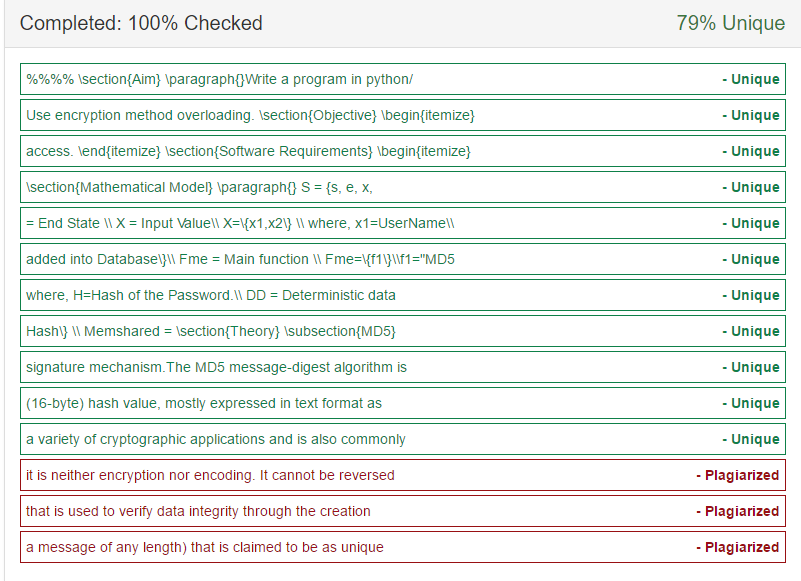
\includegraphics[width=\textwidth]{encr_plag}
\section{Output}
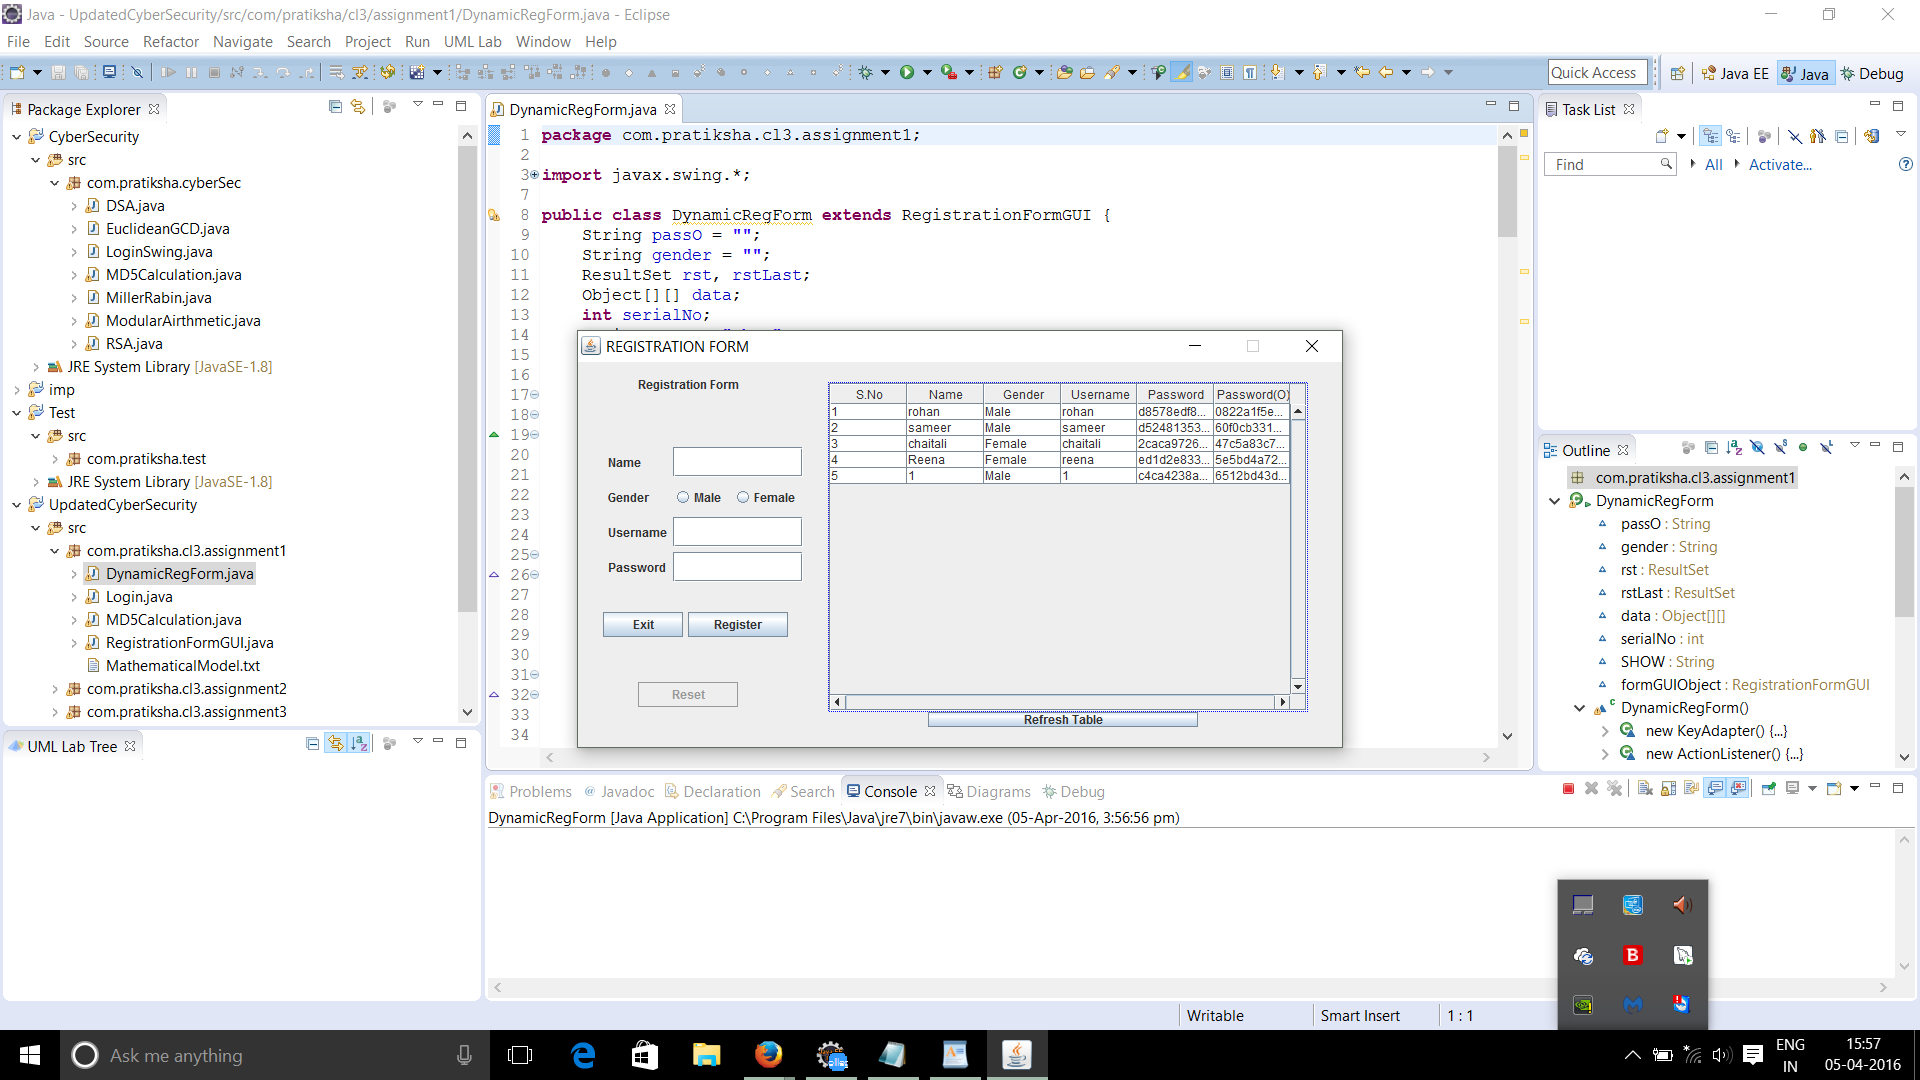
\includegraphics[width=\textwidth]{1}
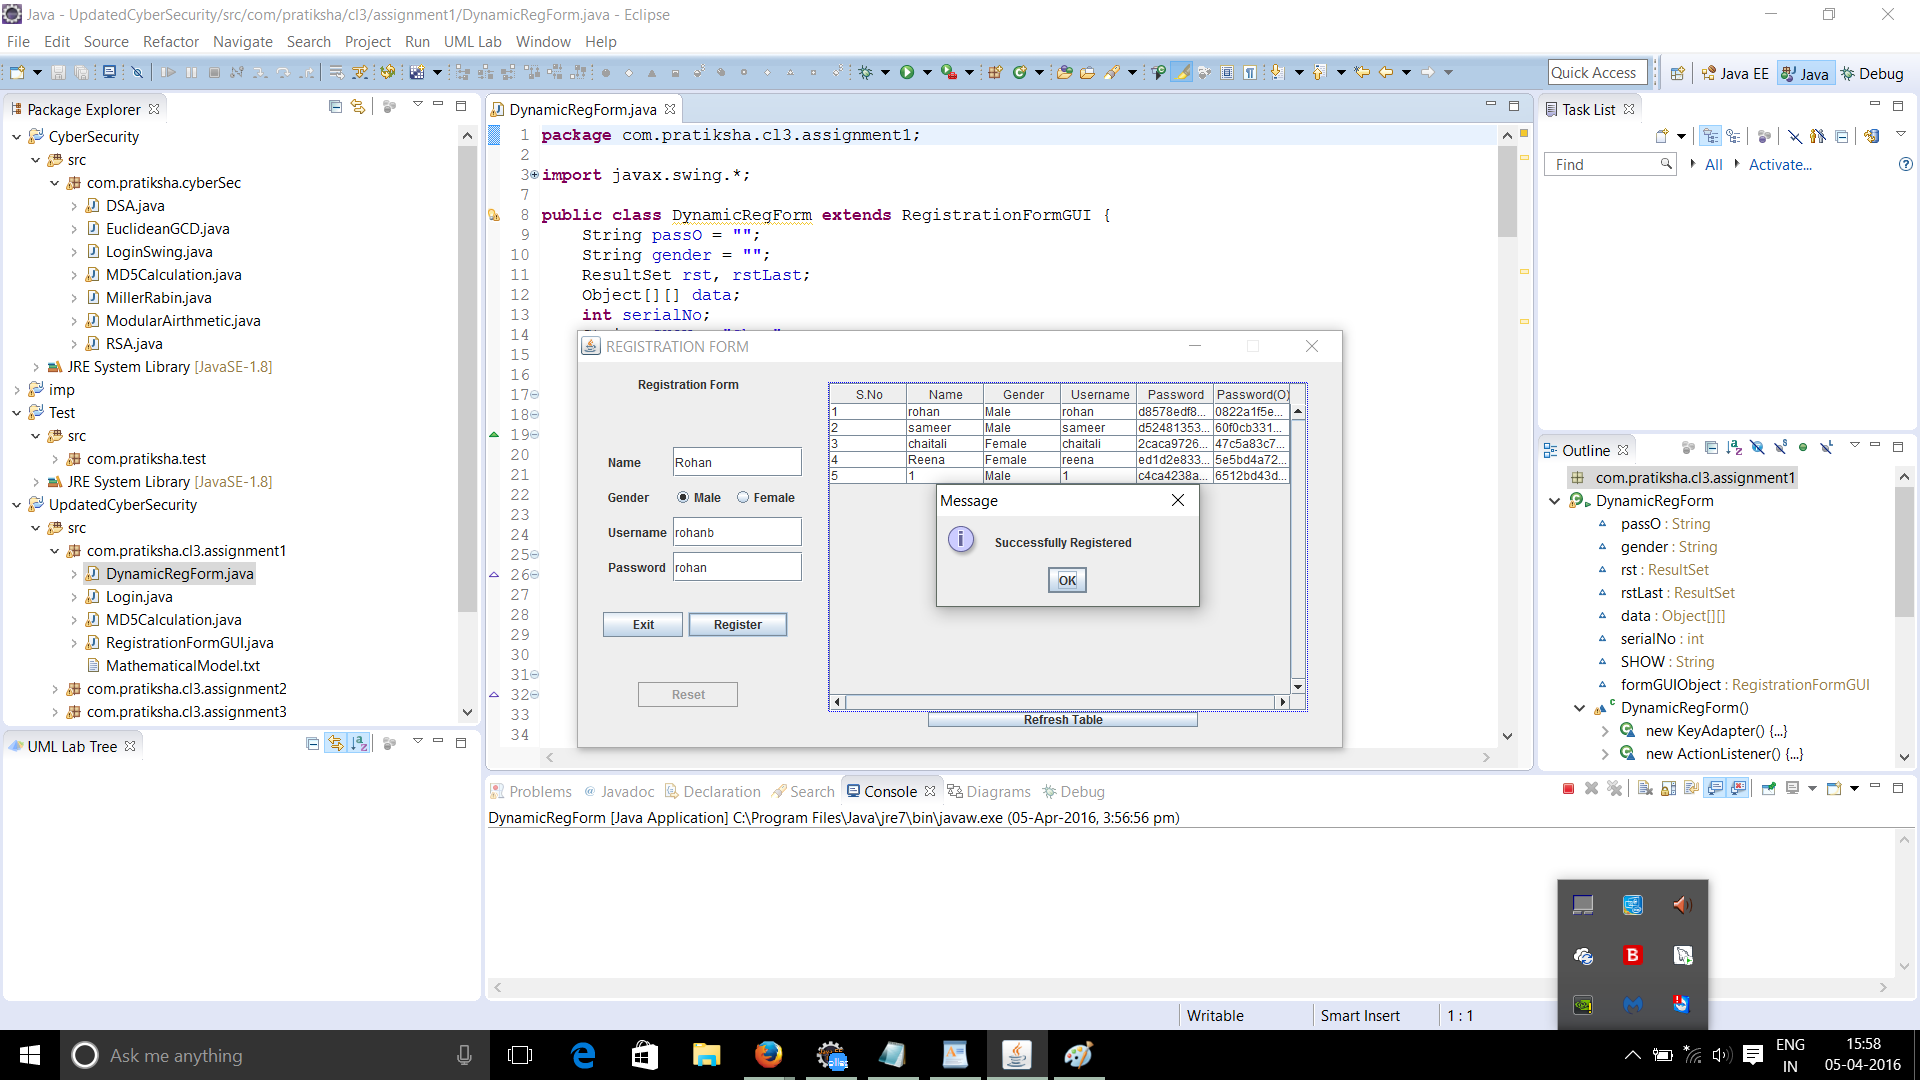
\includegraphics[width=\textwidth]{2}
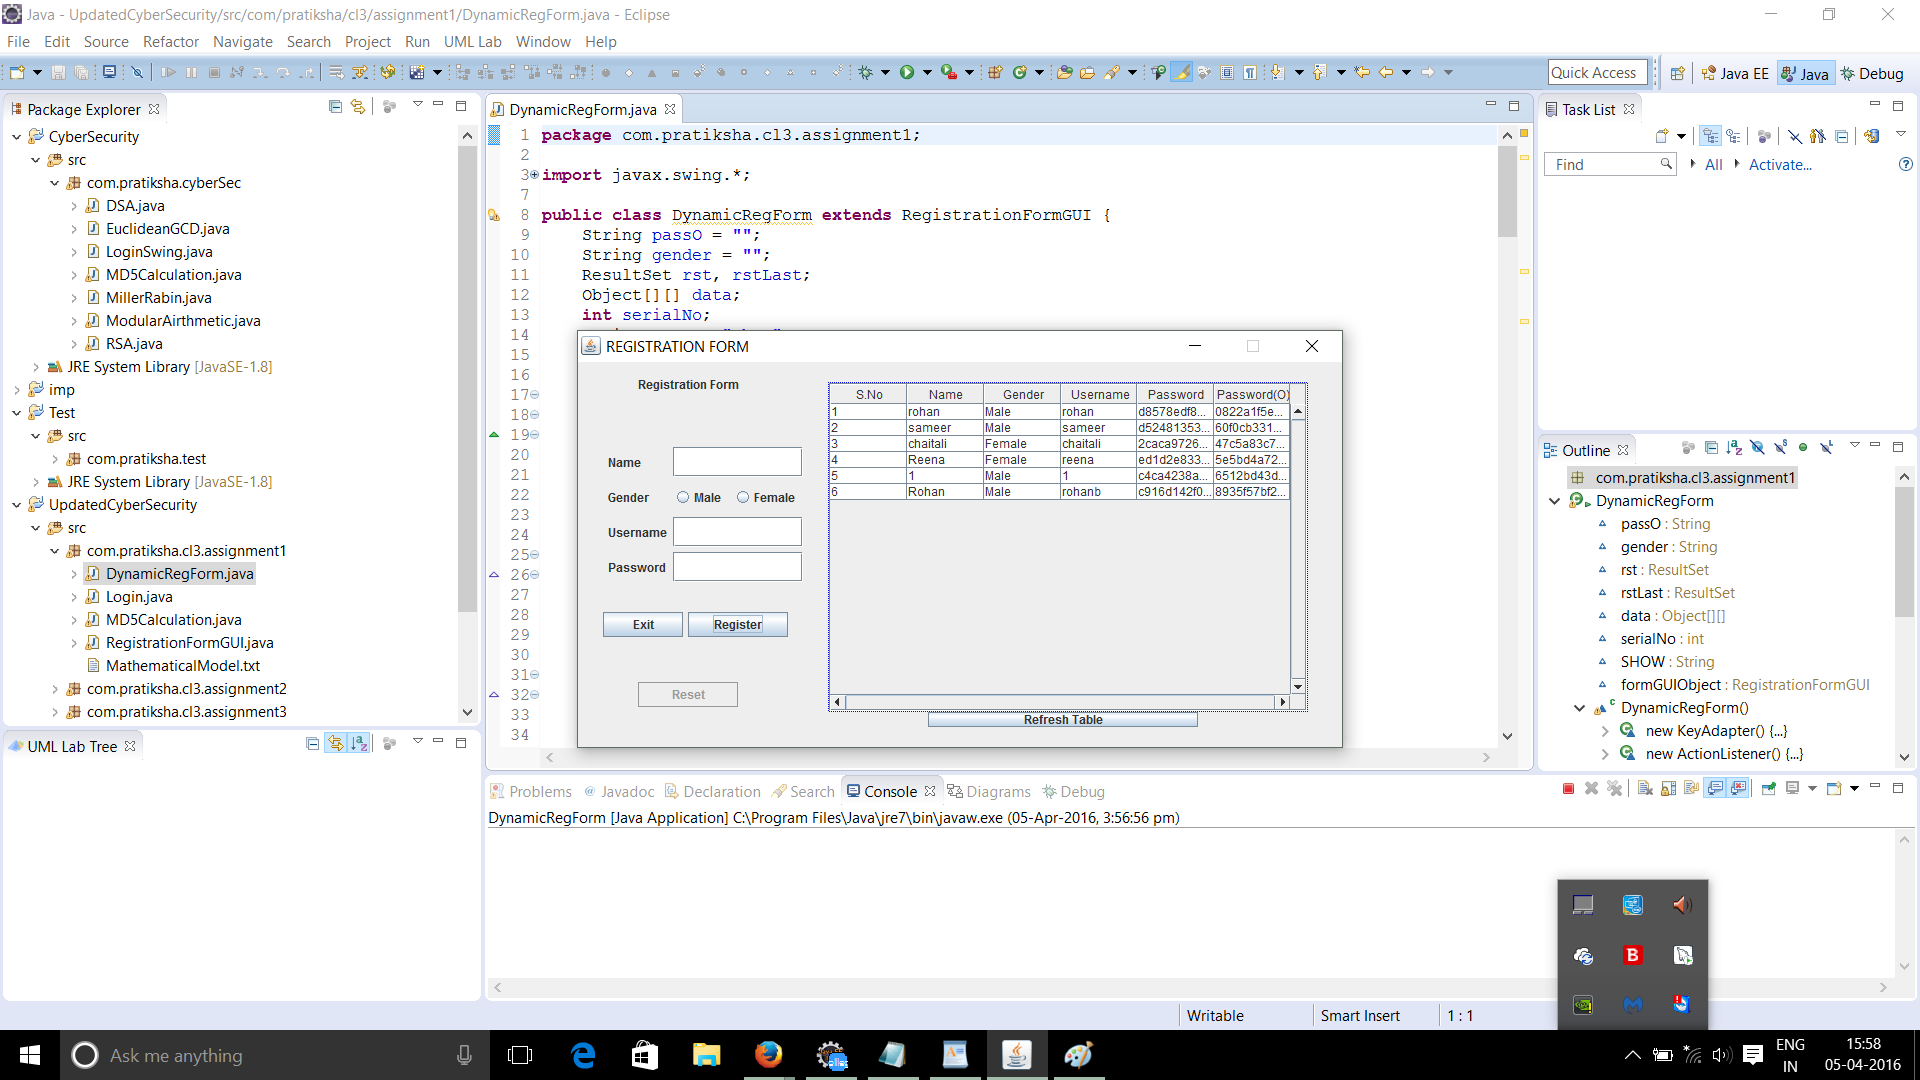
\includegraphics[width=\textwidth]{3}
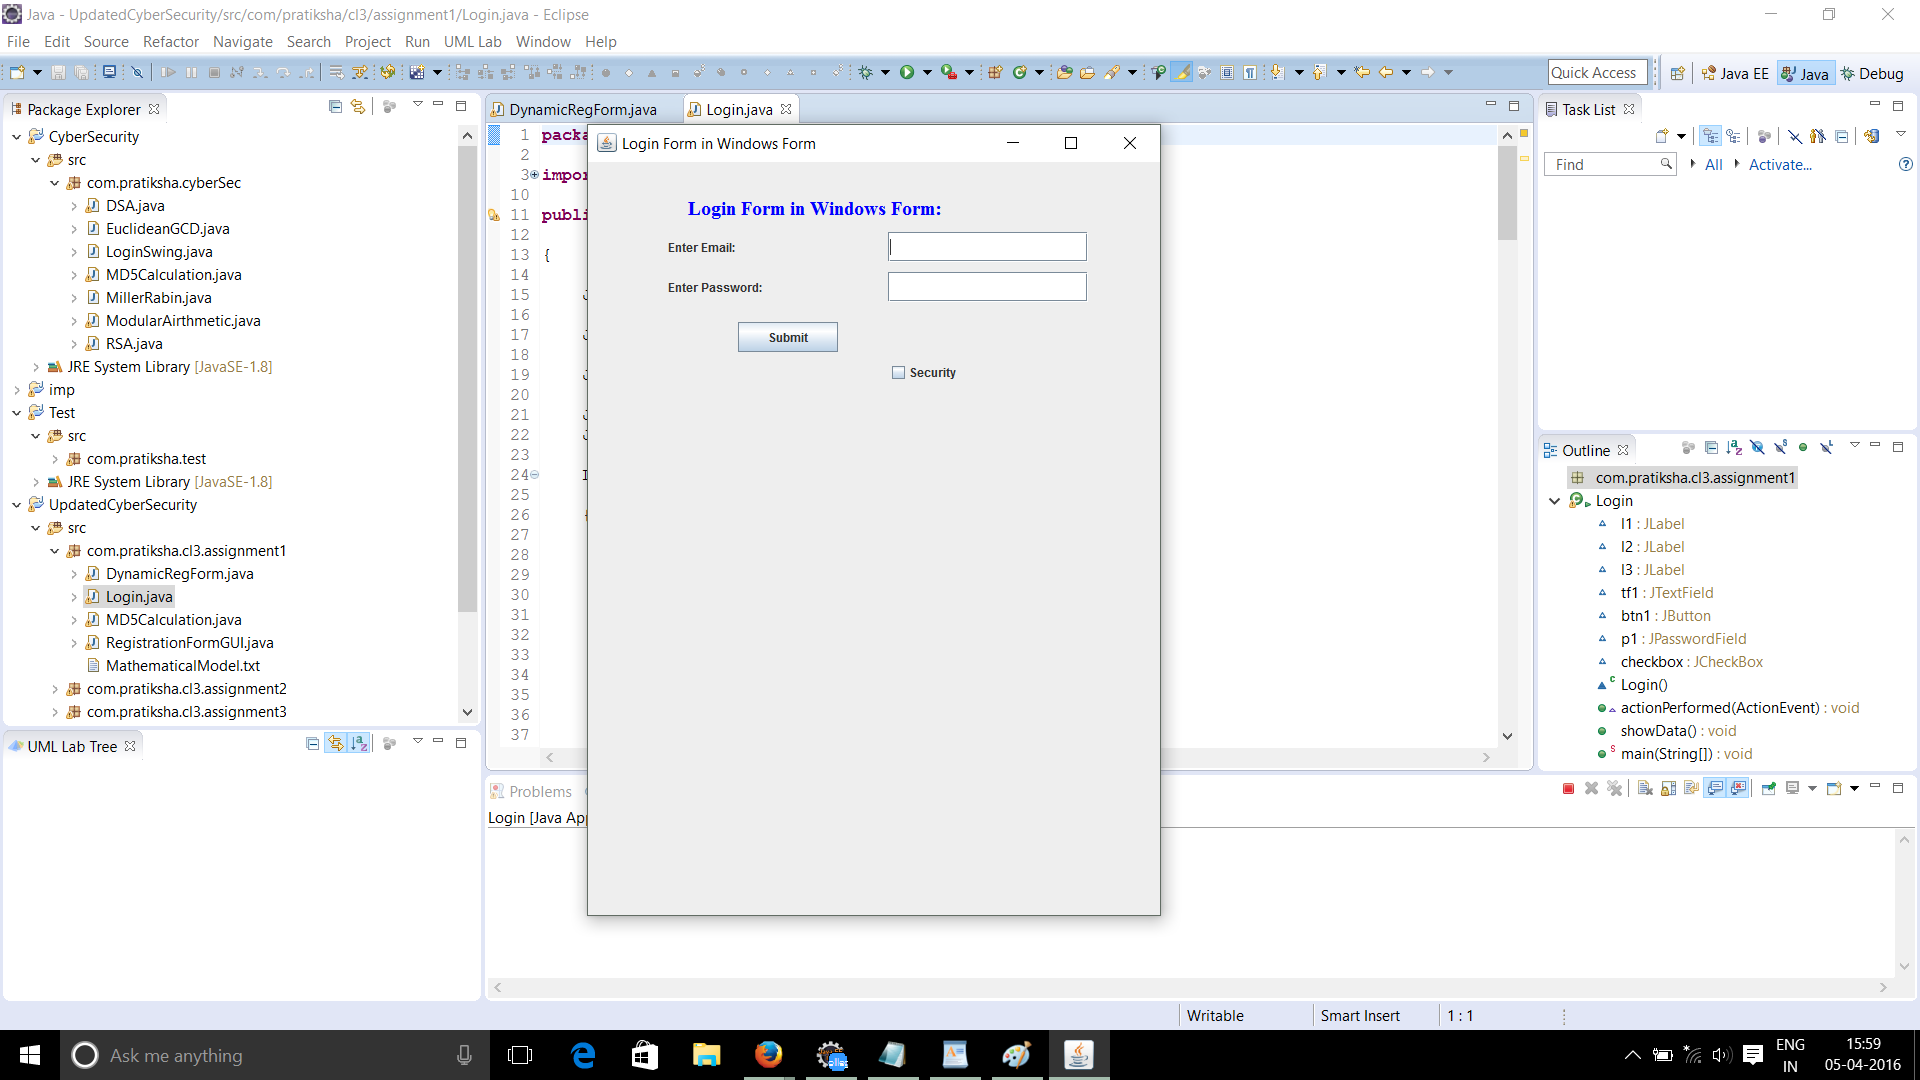
\includegraphics[width=\textwidth]{4}
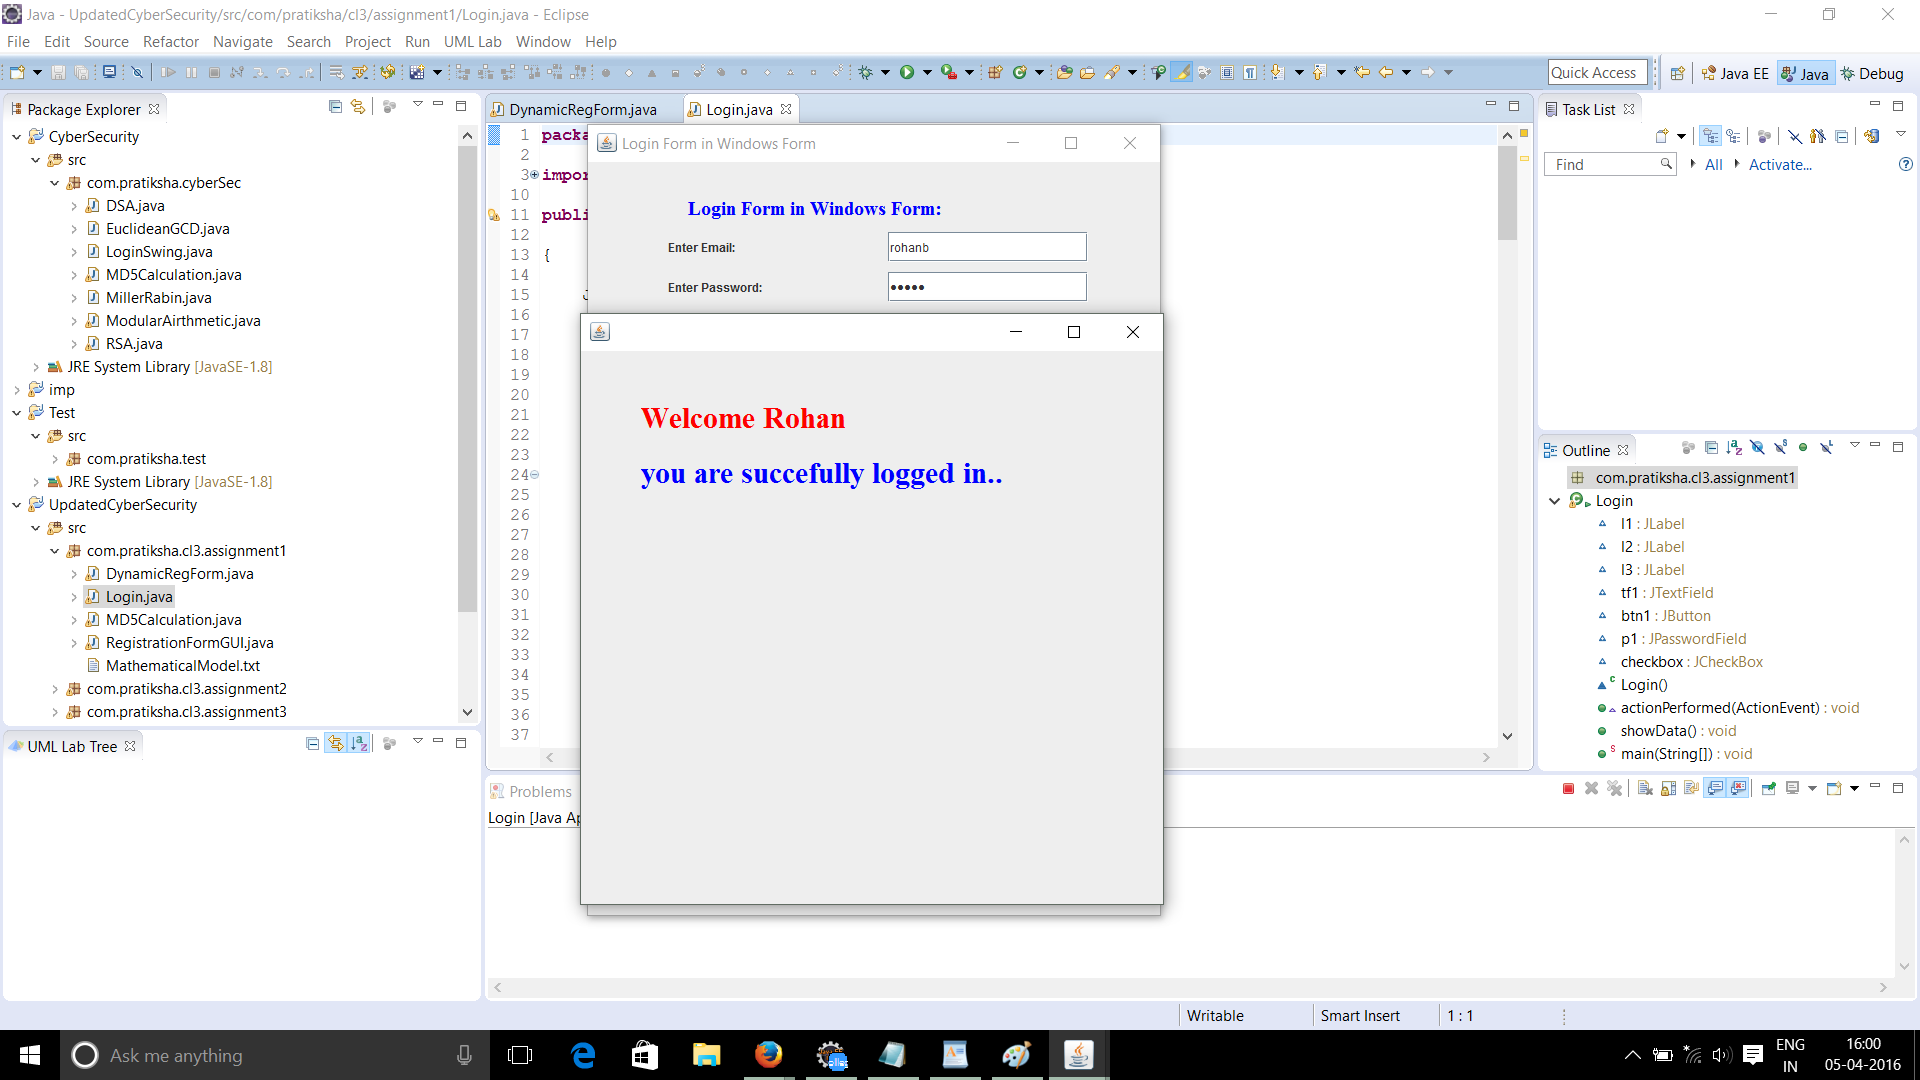
\includegraphics[width=\textwidth]{5}
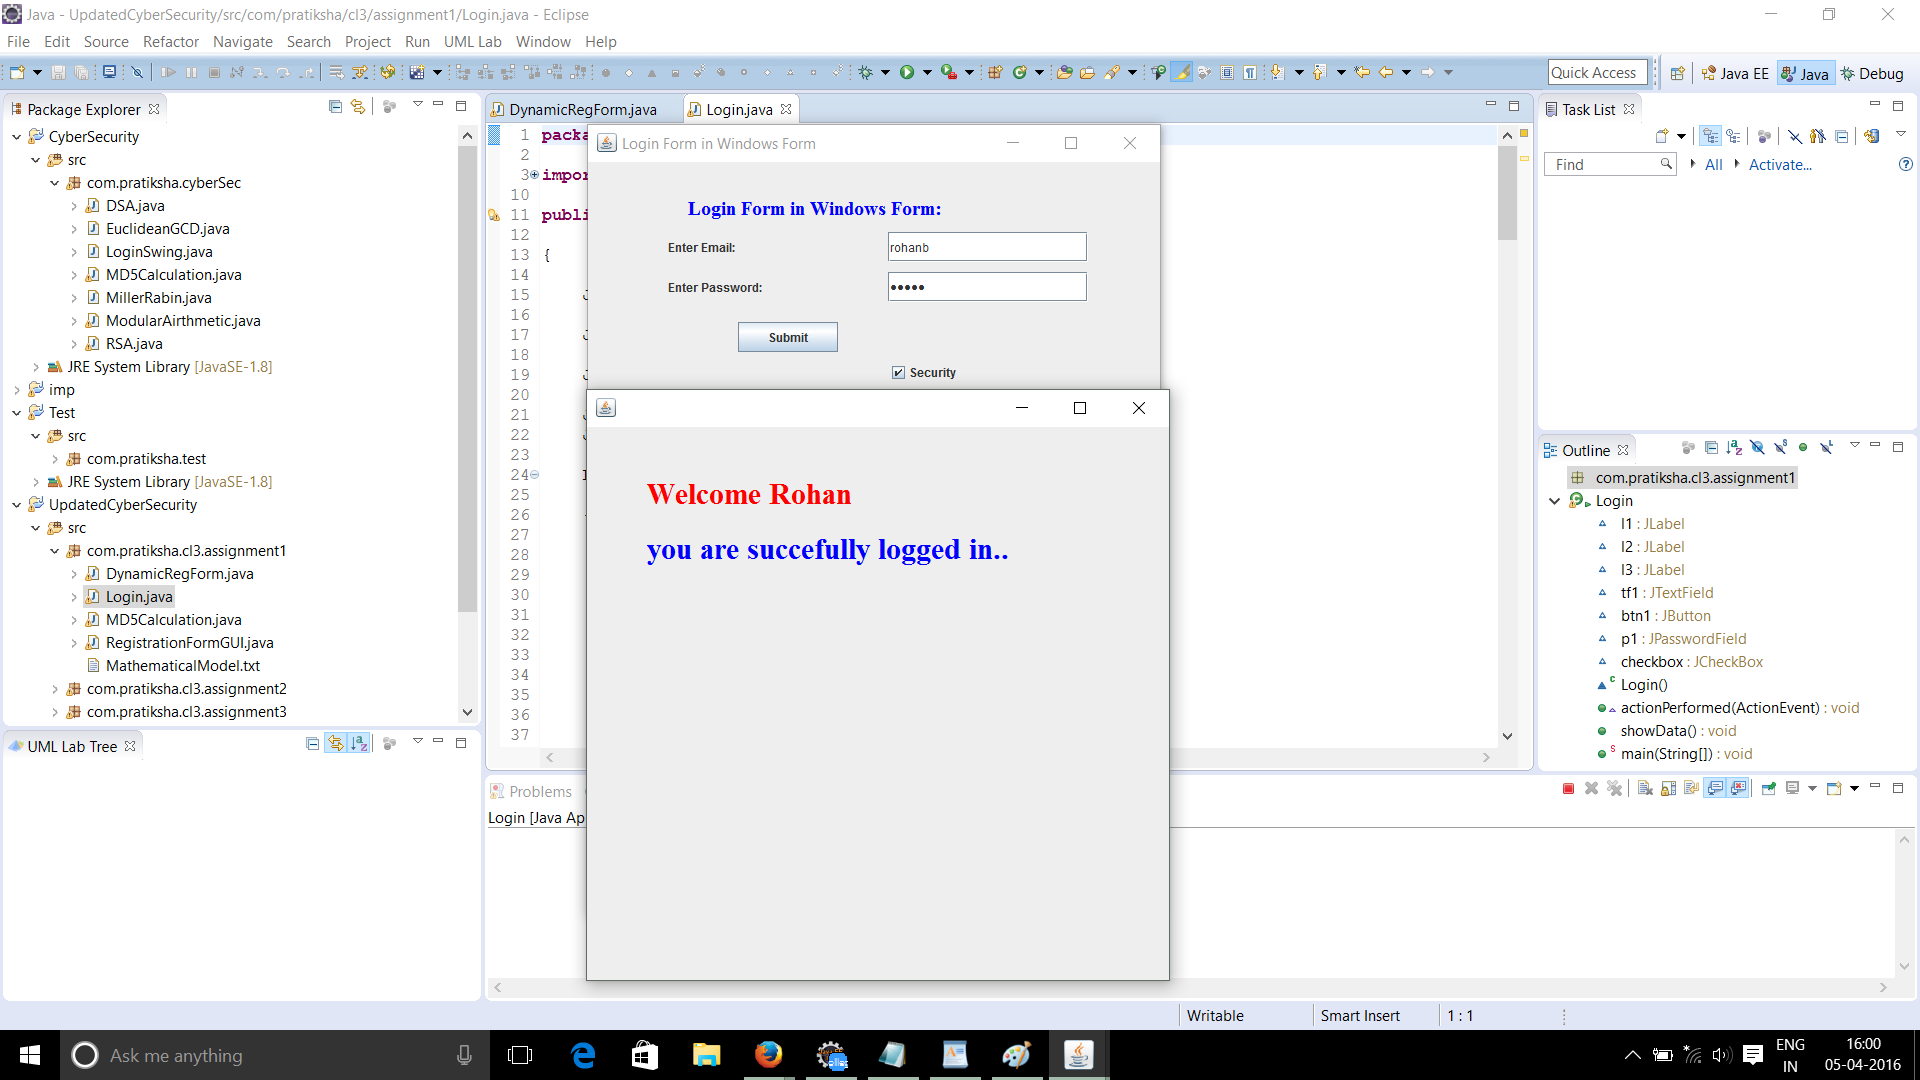
\includegraphics[width=\textwidth]{6}

\end{document}
 

 
